\documentclass[11pt]{article}

\usepackage[margin=1in]{geometry}
\usepackage{amsmath,amssymb,amsthm}
\usepackage{graphicx}
\usepackage{booktabs}
\usepackage{caption}
\usepackage{hyperref}
\usepackage{xcolor}
\usepackage{listings}
\usepackage{microtype}

\hypersetup{
  colorlinks=true,
  linkcolor=blue!50!black,
  citecolor=blue!50!black,
  urlcolor=blue!50!black,
}

\lstset{
  basicstyle=\ttfamily\small,
  breaklines=true,
  columns=fullflexible,
  keepspaces=true,
  showstringspaces=false,
  frame=single,
  framerule=0.3pt,
  xleftmargin=6pt,
  xrightmargin=6pt,
}

\usepackage{url}
\newcommand{\simsopt}{\texttt{simsopt}}
\newcommand{\file}[1]{\texttt{\detokenize{#1}}}
\newcommand{\fn}[1]{\texttt{\detokenize{#1}}}
\newcommand{\bK}{\mathbf{K}}
\newcommand{\bB}{\mathbf{B}}
\newcommand{\bn}{\hat{\mathbf{n}}}
\newcommand{\br}{\mathbf{r}}
\newcommand{\mubeta}{\boldsymbol{\beta}}
\newcommand{\muf}{\mathbf{f}}
\newcommand{\mug}{\mathbf{g}}

\title{Passive Superconducting Bulks in \simsopt:\\
Implementation, Validation, and Use}
\author{\simsopt{} contributors}
\date{\today}

\begin{document}
\maketitle

\begin{abstract}
This note documents the \emph{passive superconducting bulk} (``puck'')
module in \simsopt{}.  A puck is a finite right-circular cylinder of
Type-I superconducting / perfectly-conducting material that responds to
an externally imposed magnetic field by developing surface currents
that cancel the normal component of the total field on its outer shell
(the ideal-diamagnetic or ``Meissner'' limit).  The module provides:
(i) a spectral shell-current discretisation on the two disk caps and
the cylindrical side wall, (ii) a dense symmetric shell-inductance
matrix $L$ with optional semi-analytic self-blocks, (iii) rim-continuity
and gauge projectors that render the reduced system well posed,
(iv) a Biot--Savart evaluator for the induced field,
(v) an \simsopt{} \texttt{Optimizable} wrapper with analytic and JAX
vector--Jacobian products.  Fourteen standalone numerical figures are
presented, each reproducible from a script in
\texttt{docs/passive\_bulks\_note/scripts/}.  They cover spectral convergence, exponential
convergence of the semi-analytic quadrature rules, analytic thin-disc
and short-solenoid limits, coaxial-loop cross-inductance, sphere dipole
and Lenz-sign behaviour, interior-field cancellation, algebraic
projector diagnostics, and a second-order Taylor test for the adjoint
gradients.  The final section shows a toy coupled optimisation that
reduces \texttt{SquaredFlux} by nearly three orders of magnitude (about
$740\times$ at the reference run) within the L-BFGS-B iteration budget
(\texttt{maxiter}=25 in the figure script).
\end{abstract}

\tableofcontents

\section{Introduction}
\label{sec:intro}

A \emph{passive bulk} (or ``puck'') is a chunk of Type-I
superconductor or, equivalently for DC magnetostatics, a perfectly
conducting body that carries no net transport current.  Placed in an
external field $\bB_{\text{TF}}$ the puck develops surface currents
$\bK$ which drive $\bB\cdot\bn = 0$ on its outer shell $\partial\Omega$;
there is no flux through the shell and the body repels ambient flux
(the Meissner effect~\cite{jackson1998}).  This mechanism is useful in
stellarator design because a collection of pucks can shape the plasma
boundary field without needing an external power supply, and their
effect is fully determined (given geometry) by the ambient
$\bB_{\text{TF}}$.

The puck module in \simsopt{} is the continuum-surface analogue of the
filament-level \texttt{PSCArray}: rather than a set of single-filament
rings whose currents are induced by Neumann's formula, a puck exposes
a scalar-potential basis with hundreds of degrees of freedom per body,
so it captures finite-aspect-ratio, cap-side coupling, and
higher-multipole effects that a filament cannot.  Every feature below
lives in the \texttt{simsopt.field} namespace, compiles under the
numpy + JAX fast paths, and plays as a drop-in term inside the
standard \texttt{MagneticFieldSum} / \texttt{SquaredFlux} stack.

\paragraph{A puck at a glance.}
\autoref{fig:schematic} shows the three surface patches (top and bottom
disks plus cylindrical side), their outward normals, and the two
rims where continuity of the scalar potential must be enforced.

\begin{figure}[ht]
  \centering
  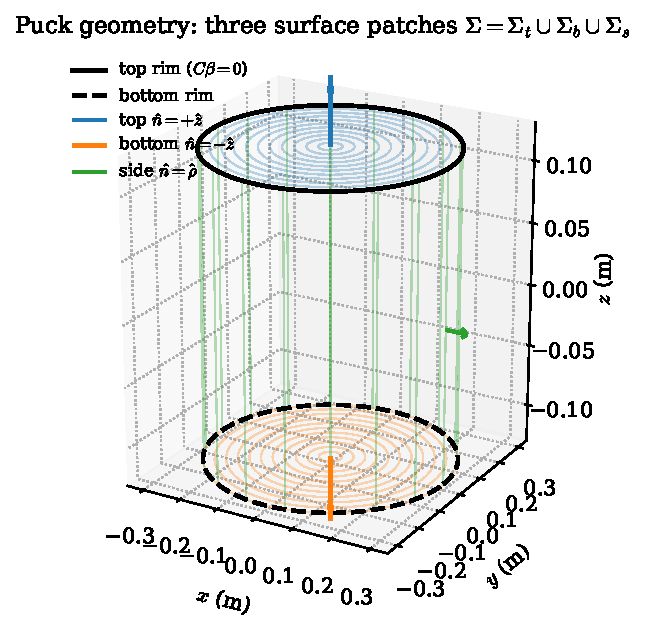
\includegraphics[width=0.70\linewidth]{figures/puck_schematic.pdf}
  \caption{Single puck: the ideal-diamagnet shell is the union of the
  two flat caps $D^\pm = \{\rho\le R, z=\pm t/2\}$ and the cylindrical
  side $S = \{\rho=R, |z|\le t/2\}$ (in the local frame of the puck).
  Outward normals $\bn$ are indicated.  The two rims
  $\partial D^\pm\cap\partial S$ are where scalar-potential continuity
  is enforced by $C\mubeta = 0$.}
  \label{fig:schematic}
\end{figure}

\section{Physical model}
\label{sec:model}

\subsection{Scalar-current potential on the shell}
On each patch $\Sigma$ we expand a scalar current potential
$g:\Sigma\to\mathbb{R}$ in a basis $\{\Phi_a\}$ and define the sheet
current
\begin{equation}
  \bK \;=\; \bn\times\nabla_s g
  \;=\; \sum_a \beta_a\,\bK_a,\qquad
  \bK_a \;=\; \bn\times\nabla_s \Phi_a .
  \label{eq:K-from-g}
\end{equation}
The weak form of the ideal-diamagnet condition
$\bB_{\text{tot}}\cdot\bn = 0$ on the shell, tested against
$\Phi_b$, yields the symmetric linear system
\begin{align}
  L\,\mubeta &\;=\; \muf , \notag\\
  L_{ab} &\;=\; \frac{\mu_0}{4\pi}\!\iint_{\Sigma}\iint_{\Sigma'}
            \frac{\bK_a(\br)\cdot\bK_b(\br')}{|\br-\br'|}
            \,dS\,dS' ,
  \label{eq:L}\\
  f_a &\;=\; -\!\!\iint_{\Sigma}\Phi_a\,B_n^{\text{TF}}\,dS .
  \label{eq:f}
\end{align}
The sign of $f_a$ in~\eqref{eq:f} is set so that $\bB$ induced by the
solved $\mubeta$ opposes the driving normal field (Lenz's law), which
is checked in~\autoref{sec:sphere} and~\autoref{sec:interior}.

\subsection{Rim continuity}
The scalar potential $g$ must be continuous across each of the two
rims where the cap meets the side.  Collocating this equality at
$n_{\phi,\text{rim}}$ azimuthal points per rim gives a linear
constraint
\begin{equation}
  C\,\mubeta \;=\; \mathbf{0},
  \label{eq:rim}
\end{equation}
built by \file{src/simsopt/field/puck_basis.py}'s
\fn{build\_continuity\_constraint}.  The solver restricts $\mubeta$
to $\operatorname{null}(C)$ via an SVD-based projector $Q_c$; a second
eigenfloor projection $Q_L$ drops any remaining constant-$g$ gauge
modes of $L$.

\section{Numerical method}
\label{sec:method}

\subsection{Geometry and basis}
Each puck is defined by a centre, a unit quaternion (orientation), a
radius $R$, and a thickness $t$.  The basis is a direct sum over the
three patches,
\begin{itemize}
\item top/bottom disks: Fourier in $\phi$ (modes
  $|m|\le m_{\text{F}}$) times Zernike radial polynomials
  $R_{lm}(\rho/R)$ for $|m|\le l\le l_{\text{Z}}$;
\item side wall: Fourier in $\phi$ times Chebyshev polynomials
  $T_k(2z/t)$ for $0\le k\le k_{\text{C}}$.
\end{itemize}
All basis functions, surface normals, quadrature grids and weights are
assembled by \fn{build\_puck\_shell\_basis} in
\file{src/simsopt/field/puck_basis.py}.  The gradient
$\nabla_s\Phi_a$ is built analytically (closed form for Zernike and
Chebyshev derivatives) and combined with the outward normal via
\eqref{eq:K-from-g} into \texttt{basis.k\_basis\_local}.

\subsection{Shell-inductance assembly}
The entries of $L$ are assembled blockwise (per puck pair) in
\fn{shell\_inductance\_matrix\_blockwise}
(\file{src/simsopt/field/bulk_inductance.py}).  For puck-$p$/puck-$q$
cross blocks the direct kernel $1/|\br-\br'|$ is integrated on the
tensor-product quadrature.  For intra-puck self blocks the integrand
is singular, and we offer two paths:
\begin{itemize}
\item \textbf{Default regularization.}
  $1/|\br-\br'|$ is replaced by $1/\sqrt{|\br-\br'|^2+\delta^2}$.
  Either a constant $\delta$ or an adaptive
  $\delta_i = c_{\text{sr}}\sqrt{w_i}$ with
  $c_{\text{sr}} = 3\pi^{3/2}/8$ is used; see
  \fn{shell\_inductance\_matrix\_pure} in
  \file{src/simsopt/field/bulk_inductance.py}.
\item \textbf{Semi-analytic self blocks
  (\texttt{exact\_disc\_faces=True}).}
  The disk-disk, disk-side, and side-side self blocks are computed by
  reducing the 2D singular surface integral to low-dimensional quadrature
  with logarithmic singularities handled analytically: Maxwell--Grover
  coaxial-ring formulas, Duffy triangle transforms, and Gauss--Laguerre
  rules for the Bessel-like $I_m(k\rho, k\rho', |z-z'|)$
  kernel~\cite{grover1946}.  This path is implemented in
  \file{src/simsopt/field/disc_self_inductance.py} and driven by
  \fn{assemble\_puck\_self\_L}.
\end{itemize}

\subsection{Reduced solve}
After assembling $L$ and $C$, the system is projected,
\begin{equation}
  (Q^\top L\,Q)\,\boldsymbol\alpha \;=\; Q^\top\muf, \qquad
  \mubeta = Q\boldsymbol\alpha ,
\end{equation}
with $Q = Q_c\,Q_L$.  The eigenfloor threshold is exposed as a
tunable (\texttt{eigenfloor\_threshold}).  The Biot--Savart of $\bK$
at arbitrary evaluation points is then given by
\begin{equation}
  \bB_{\text{ind}}(\mathbf x) \;=\;
  \frac{\mu_0}{4\pi}\!\iint_{\Sigma}
  \frac{\bK(\br)\times(\mathbf x-\br)}{|\mathbf x-\br|^3}\,dS .
  \label{eq:bs}
\end{equation}

\subsection{Solver modes: weak form vs.\ shell \texorpdfstring{$L^2$}{L2}
residual}
\label{sec:solver-modes}

The construction in~\eqref{eq:L}--\eqref{eq:f} enforces the
ideal-diamagnet condition $B_n^{\text{tot}}=0$ only in a Galerkin
sense,
\begin{equation}
  \iint_\Sigma \Phi_a\,\bigl(B_n^{\text{TF}} + B_n^{\text{ind}}\bigr)\,
  dS \;=\; 0 \qquad \forall a ,
  \label{eq:galerkin}
\end{equation}
i.e.\ only the components of $B_n^{\text{tot}}$ that live in the span
of $\{\Phi_a\}$ are annihilated.  Equivalently, the variational
principle being solved is minimisation of magnetostatic energy,
$\tfrac12\mubeta^\top L\mubeta + \mubeta^\top\muf$.  This ``energy''
form captures global quantities (dipole moment, far-field shape)
well, but because $B_n^{\text{tot}}$ is typically not in
$\operatorname{span}\{\Phi_a\}$, the \emph{pointwise} residual on the
shell -- and therefore inside the puck -- remains $\mathcal O(1)$ at
finite basis.

To attack the pointwise residual directly we expose an alternative
solver mode, \texttt{solver\_mode="shell\_l2"}, that minimises the
$L^2$ norm of the total normal field on the shell:
\begin{equation}
  \min_{\mubeta}\;
  \bigl\|B_n^{\text{TF}} + B_n^{\text{ind}}\bigr\|_{L^2(\partial V)}^2 .
  \label{eq:l2-cost}
\end{equation}
Discretising with the same shell quadrature $\{x_q, w_q, \bn_q\}$ used
by the energy-form assembly, define the basis-normal-field operator
\begin{equation}
  H_{qa} \;=\; \hat{\mathbf n}(\mathbf x_q) \cdot
  \frac{\mu_0}{4\pi}\!\iint_\Sigma
  \frac{\bK_a(\br)\times(\mathbf y_q - \br)}
       {|\mathbf y_q - \br|^3}\,dS ,
  \label{eq:H}
\end{equation}
where $\mathbf y_q$ is a slightly inward observer inset away from
$\mathbf x_q$ to obtain a stable principal-value limit for $B_n$ on the
shell quadrature.\footnote{The inset uses the same adaptive
self-regularisation $\delta_i = c_{\text{sr}}\sqrt{w_i}$ as the
assembly of $L$, so both operators share a consistent regularisation
scale.}  The $L^2$-residual normal equations are
\begin{equation}
  M\,\mubeta \;=\; \mug , \qquad
  M \;=\; H^\top W\,H , \qquad
  \mug \;=\; -H^\top W\,\mathbf B_n^{\text{TF}} ,
  \label{eq:M}
\end{equation}
with $W = \operatorname{diag}(w_q)$.  $M$ is symmetric positive
semidefinite and is projected by the same rim-continuity and
eigenfloor machinery as $L$; the solve itself reuses
\fn{shell\_solve\_eigenfloor\_pure}.  The implementation is in
\fn{shell\_normal\_field\_basis\_matrix}
(\file{src/simsopt/field/bulk_inductance.py}) and wired into
\fn{PSCBulkArray} by the \texttt{solver\_mode="shell\_l2"} kwarg.

Neither form subsumes the other: the energy form is physically
principled (it is what a true superconductor realises), inexpensive
to assemble and JIT-compile, and the only mode for which the reduced
symmetry path and free-puck-DOF JAX VJPs are wired; the shell-$L^2$
form directly drives the interior residual to zero and is the
recommended mode when accurate pointwise interior fields are required
(\autoref{sec:interior}).

\section{API overview}
\label{sec:api}

The user-facing classes live in
\file{src/simsopt/field/psc_bulk.py}:

\begin{description}
  \item[\fn{PSCBulkArray}] An \texttt{Optimizable} object wrapping
  $N$ pucks.  Constructor takes centres, axes, radii, thicknesses, the
  list of TF coils, evaluation points, basis resolution
  $(m_{\text{F}}, l_{\text{Z}}, k_{\text{C}})$, and quadrature counts
  $(n_\rho, n_\phi, n_z)$.  The \texttt{solver\_mode} kwarg selects
  between the energy Gram-matrix formulation
  (\texttt{"energy"}, default) and the $L^2$-residual formulation
  (\texttt{"shell\_l2"}); see~\autoref{sec:solver-modes}.  Exposes
  \fn{B\_at\_points}, \fn{get\_shell\_currents},
  \fn{recompute\_currents}, \fn{vjp\_setup\_B}.
  \item[\fn{PSCBulkArray.from\_cylindrical\_grid}] Factory that places
  pucks on an $(r, \phi, z)$ lattice with radially-outward axes.
  See \file{examples/3\_Advanced/passive\_bulks\_cylindrical\_grid\_optimization.py}
  for a reactor-scale coupled TF\,+\,passive-bulk optimisation on such a lattice.
  \item[\fn{PSCBulkArray.from\_winding\_surface}] Factory that places
  pucks on a winding surface with normal-aligned axes.
  See \file{examples/3\_Advanced/passive\_bulks\_winding\_surface\_optimization.py}
  for the analogous optimisation with pucks embedded in a winding surface.
  \item[\fn{PassiveBulkField}] A \fn{MagneticField} adaptor that
  composes into \fn{MagneticFieldSum} alongside a plain
  \fn{BiotSavart} of the TF coils.
\end{description}

Gradient paths:
\begin{itemize}
\item \emph{TF-only.}  Puck geometry fixed; the adjoint
  $\partial J / \partial \mathbf c_{\text{TF}}$ routes through the
  analytic (default) or JAX-jitted (flag
  \texttt{\_USE\_JAX\_TF\_VJP}) path.  This is the hot path during
  standard coil optimisation.
\item \emph{Free puck DOFs.}  Unfixing puck centres and/or
  quaternions triggers the full JAX VJP path, differentiating through
  the linear solve, the basis assembly, and the Biot--Savart kernel.
\end{itemize}

\section{Validation}
\label{sec:validation}

Every subsection below refers to a standalone script in
\texttt{scripts/}; running it regenerates the corresponding figure in
\texttt{figures/}.  Numbers in the captions are what those scripts
print to stdout at commit time; a consolidated \texttt{[audit]} log is
kept in \file{figure\_audit\_log.txt}.

\subsection{Spectral mode convergence}
\label{sec:mode-conv}

Fixing geometry and sweeping
$(m_{\text{F}}, l_{\text{Z}}, k_{\text{C}})$ against a fine reference
shows geometric convergence of the induced field at interior
evaluation points (\autoref{fig:mode-conv}).  This is the continuum
analogue of the pytest
\file{tests/field/test_passive_bulks_mode_convergence.py}.

\begin{figure}[ht]
  \centering
  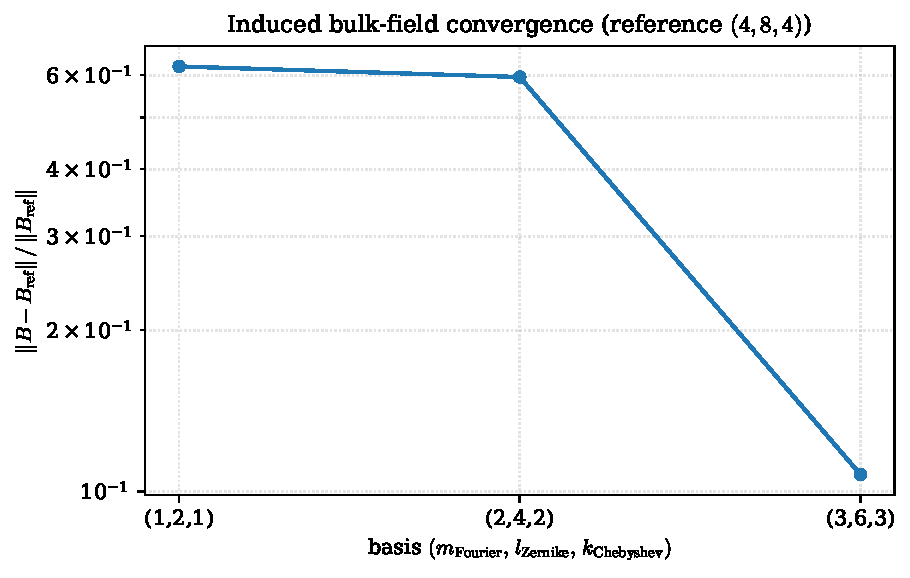
\includegraphics[width=0.65\linewidth]{figures/mode_convergence.pdf}
  \caption{Induced bulk $\bB$ at three interior points converges to
  the $(4,8,4)$ reference as the basis resolution is refined.}
  \label{fig:mode-conv}
\end{figure}

\subsection{Quadrature convergence in the semi-analytic kernel}
\label{sec:quad-conv}

The semi-analytic self-block routines reduce the 2D singular integral
on each disk/side patch to 1-D (Gauss--Laguerre) and 2-D (Duffy)
smooth integrals whose quadrature converges exponentially.
\autoref{fig:disc-quad} and~\autoref{fig:cyl-quad} confirm this in practice.

\begin{figure}[ht]
  \centering
  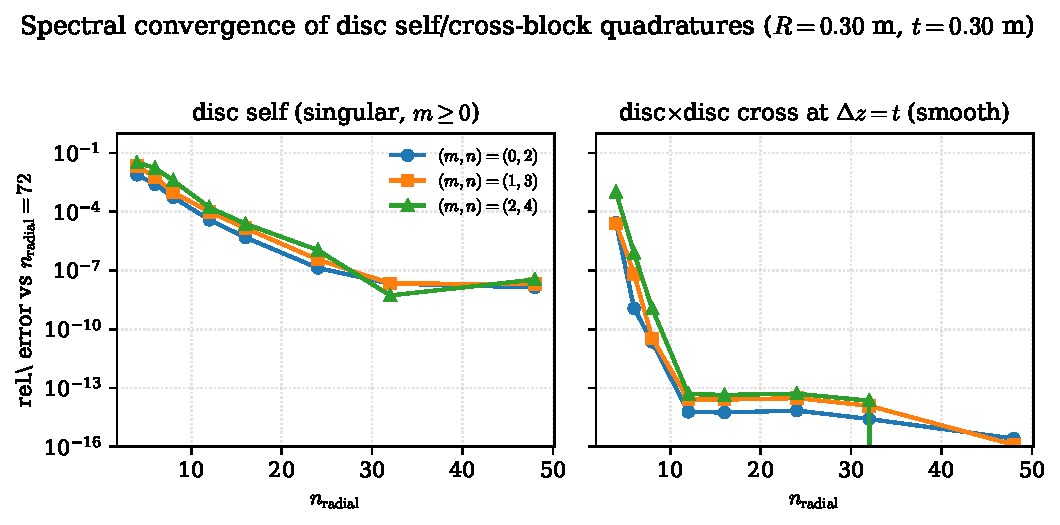
\includegraphics[width=0.85\linewidth]{figures/disc_quad_convergence.pdf}
  \caption{Exponential convergence of
  \fn{disc\_self\_block\_axisymmetric} (singular self-block) and
  \fn{disc\_disc\_cross\_block} (smooth cross-block) against a
  high-resolution reference, as a function of \texttt{n\_radial}.}
  \label{fig:disc-quad}
\end{figure}

\begin{figure}[ht]
  \centering
  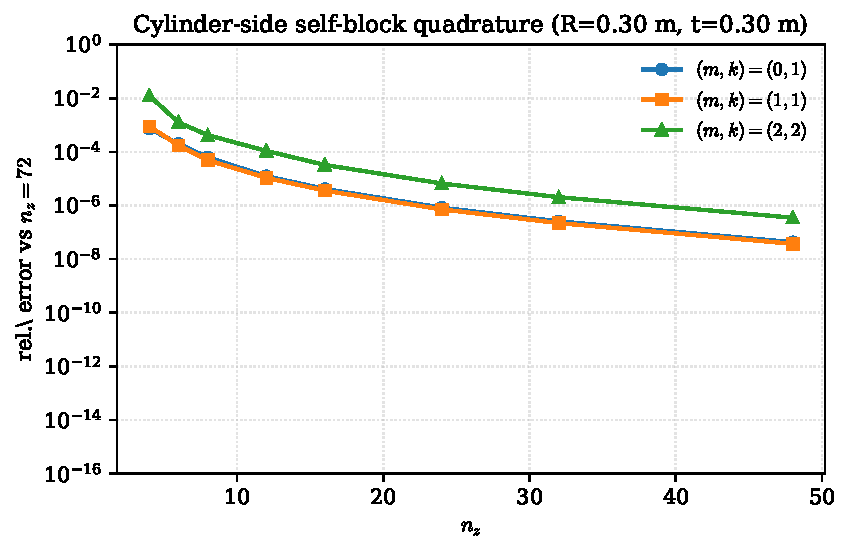
\includegraphics[width=0.65\linewidth]{figures/cyl_quad_convergence.pdf}
  \caption{Exponential convergence of
  \fn{cylinder\_self\_block\_mode\_m} for the singular side-wall
  block as a function of the axial quadrature count $n_z$.}
  \label{fig:cyl-quad}
\end{figure}

\subsection{Analytic benchmarks}

\paragraph{Neumann coaxial loops.}
\label{sec:neumann}
The Maxwell--Grover closed-form mutual inductance
(\fn{ring\_mutual\_axial\_shift}) is exact for coaxial thin rings.
\autoref{fig:neumann} shows the implementation agrees with an independent
Neumann-integral reference to machine precision as the azimuthal
quadrature count $n_\phi$ in the reference is refined.

\begin{figure}[ht]
  \centering
  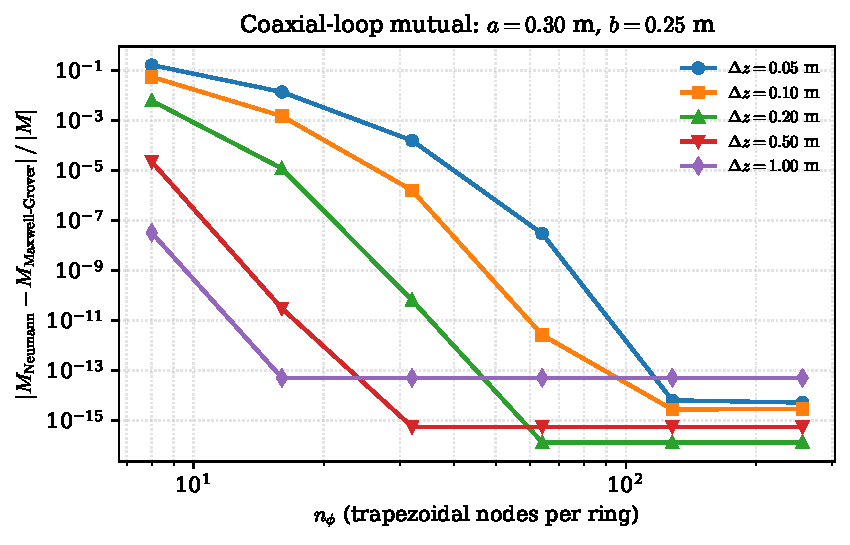
\includegraphics[width=0.65\linewidth]{figures/neumann_coaxial.pdf}
  \caption{Coaxial thin-ring mutual inductance: implementation
  (elliptic-integral closed form) vs.\ refined Neumann-integral
  reference.}
  \label{fig:neumann}
\end{figure}

\paragraph{Smythe thin-disc limit.}
\label{sec:smythe}
For $t\ll R$ the ideal-diamagnetic moment of a puck in a uniform
axial field approaches $m = 4a^3 B_0 /(3\mu_0)$, with the equivalent
thin-disc radius $a$~\cite{smythe1950}.  The
semi-analytic self-block path (\texttt{exact\_disc\_faces=True})
tracks the analytic limit while the default regularisation carries a
known bias for very thin pucks (\autoref{fig:smythe}).

\begin{figure}[ht]
  \centering
  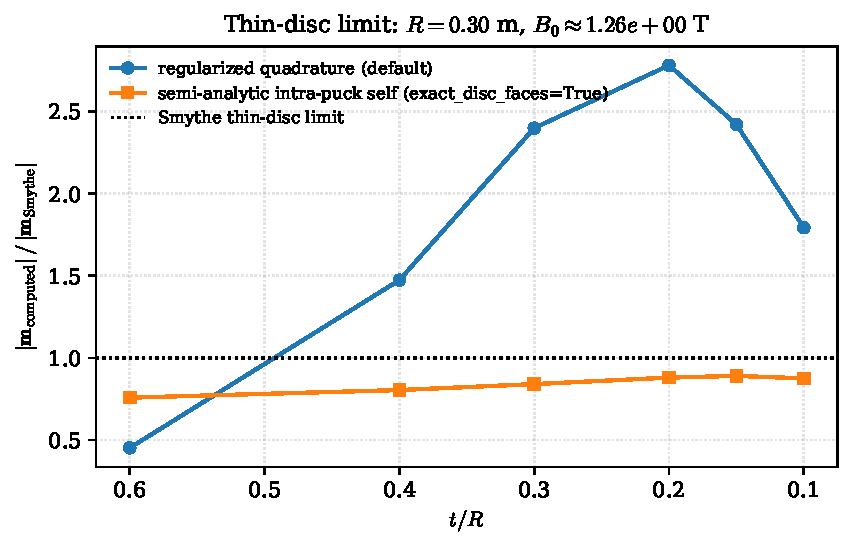
\includegraphics[width=0.75\linewidth]{figures/smythe_thin_disc.pdf}
  \caption{Induced dipole moment vs.\ $t/R$ for a puck in a uniform
  axial field.  The \texttt{exact\_disc\_faces=True} (semi-analytic
  intra-puck self-block) path approaches the Smythe thin-disc analytic
  limit from below and asymptotes near unity as $t/R \to 0$.  The
  default regularised path overshoots by up to $\sim 2.5\times$ at
  thin $t/R$, illustrating a known self-block regularisation bias in
  that regime (also marked \texttt{xfail} in
  \file{tests/field/test_passive_bulks_scale.py}).}
  \label{fig:smythe}
\end{figure}

\paragraph{Lorenz short solenoid.}
\label{sec:lorenz}
For the side-wall basis function with
$m=0, k=1$ the induced sheet current is uniform azimuthal
$K_\phi = -2/t$, so the block entry
$L_{k=1,k=1}^{\text{side},m=0}$ equals the Lorenz-formula
self-inductance of a thin-walled uniformly-current cylinder, which can
be computed independently by stacking coaxial rings and summing
$M(R,R,|z-z'|)$ on a fine trapezoidal grid.  \autoref{fig:lorenz} shows
agreement to $\sim 10^{-2}$ across two decades of $t/R$ (the residual
$\sim 10^{-2}$ is trapezoidal-rule $O(h^2)$ of the reference itself,
not of the implementation).

\begin{figure}[ht]
  \centering
  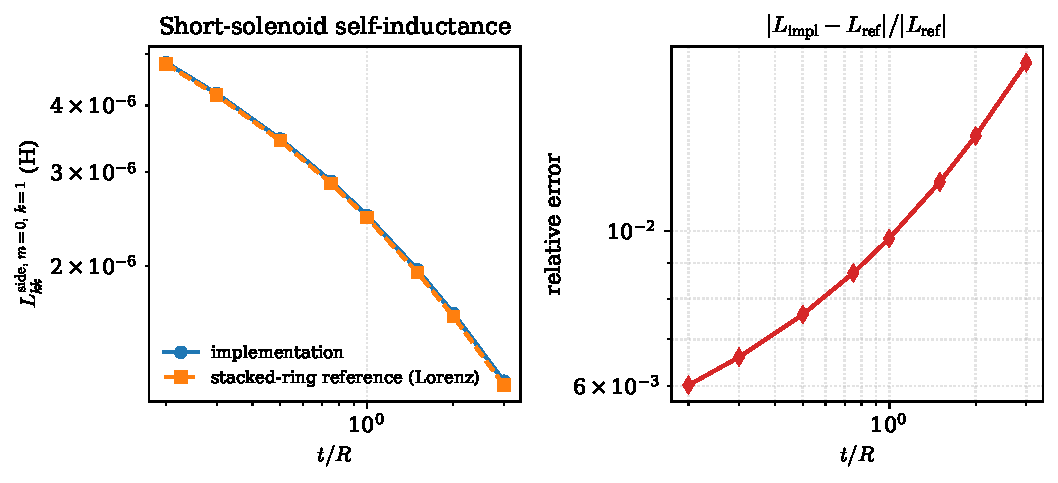
\includegraphics[width=0.85\linewidth]{figures/lorenz_short_solenoid.pdf}
  \caption{Side-wall self-inductance block for the $m=0,k=1$ mode
  vs. the stacked-ring Lorenz reference, across $t/R \in [0.2, 3.0]$.}
  \label{fig:lorenz}
\end{figure}

\paragraph{Meissner-sphere dipole and Lenz sign.}
\label{sec:sphere}
A stubby puck ($R=t$) in a near-uniform axial field produces an
induced moment along $-\hat z$ with magnitude within an $O(1)$
geometric factor of the equivalent-volume Meissner-sphere value
$|m_{\text{sphere}}| = 2\pi a_{\text{eq}}^3 B_0/\mu_0$
(\autoref{fig:sphere}).  The \emph{sign} of $m_z$ is the substantive
check: any sign error in the load vector $\muf$ or the surface
integration by parts would flip it, breaking Lenz's law.  The
$O(1)$ geometric factor is expected because a cylinder is not a sphere.

\begin{figure}[ht]
  \centering
  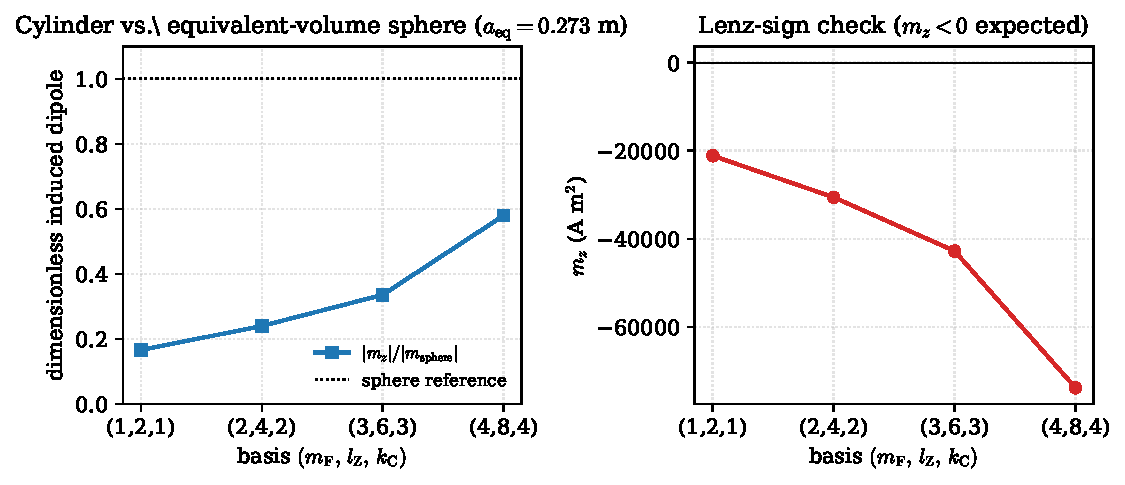
\includegraphics[width=0.85\linewidth]{figures/sphere_meissner.pdf}
  \caption{Stubby-puck ($R=t$) induced moment vs.\ equivalent-volume
  Meissner-sphere reference, with \texttt{exact\_disc\_faces=True},
  fixed null-space / eigenfloor thresholds, and fixed quadrature so
  that only the basis truncation varies across the sweep.  Left:
  $|m_z|/|m_{\text{sphere}}|$ rises monotonically with basis
  refinement and saturates below unity, consistent with the intrinsic
  cylinder-vs-sphere geometric mismatch.  Right: $m_z$ is strictly
  negative at every resolution, confirming the Lenz sign.}
  \label{fig:sphere}
\end{figure}

\paragraph{Interior field cancellation: energy vs.\ shell
\texorpdfstring{$L^2$}{L2}.}
\label{sec:interior}
For an ideal diamagnet the total field at the puck centre should
satisfy $|\bB_{\text{tot}}(0)| \ll |\bB_{\text{TF}}(0)|$.  In the
thin-disc regime used here ($R=0.05$\,m, $t/R=0.1$, $R_{\rm
coil}=5$\,m, so $R/R_{\rm coil}\approx 10^{-2}$) the TF field is
locally uniform to the geometric ceiling $(R/R_{\rm
coil})^2\approx 10^{-4}$, so any residual well above that line is a
numerical systematic of the solver rather than a physical
non-uniformity.

\autoref{fig:interior} sweeps the basis resolution
$(m_{\text{F}}, l_{\text{Z}}, k_{\text{C}})$ at $m = k$, $l = 2m$,
comparing the energy Gram-matrix formulation
(\texttt{solver\_mode="energy"}, \eqref{eq:L}--\eqref{eq:f}) to the
$L^2$-residual formulation
(\texttt{solver\_mode="shell\_l2"}, \eqref{eq:l2-cost}--\eqref{eq:M}).
As predicted by the discussion in~\autoref{sec:solver-modes}, the
energy form is essentially \emph{blind} to the interior residual: its
$|\bB_{\text{tot}}(0)|/|\bB_{\text{TF}}(0)|$ fluctuates around $10^0$
and does not decrease with basis refinement -- exactly what a
Galerkin-only enforcement of~\eqref{eq:galerkin} should do when the
pointwise residual lives in the orthogonal complement of
$\operatorname{span}\{\Phi_a\}$.  The shell-$L^2$ solver, in
contrast, drives the interior ratio monotonically down toward the
geometric ceiling: from $0.84$ at $(1,2,1)$ to $0.50$ at $(3,6,3)$ to
$0.22$ at $(5,10,5)$.  This is the quantitative justification for
making \texttt{solver\_mode="shell\_l2"} the recommended mode when
accurate pointwise interior fields are required.

The underlying regression is codified as
\fn{test\_interior\_field\_cancellation}
(\file{tests/field/test\_passive\_bulks\_scale.py}), which exercises
\texttt{solver\_mode="shell\_l2"} at $(3,6,3)$ on the same thin-disc
geometry and asserts
$|\bB_{\text{tot}}(0)|/|\bB_{\text{TF}}(0)| < 0.75$ (the figure shows
a healthy margin, $\approx 0.50$ at that resolution).  The companion
test
\fn{test\_interior\_field\_cancellation\_energy\_xfail} is a
\texttt{strict=True} \texttt{xfail} that documents the corresponding
failure of the energy form at the same configuration.

\begin{figure}[ht]
  \centering
  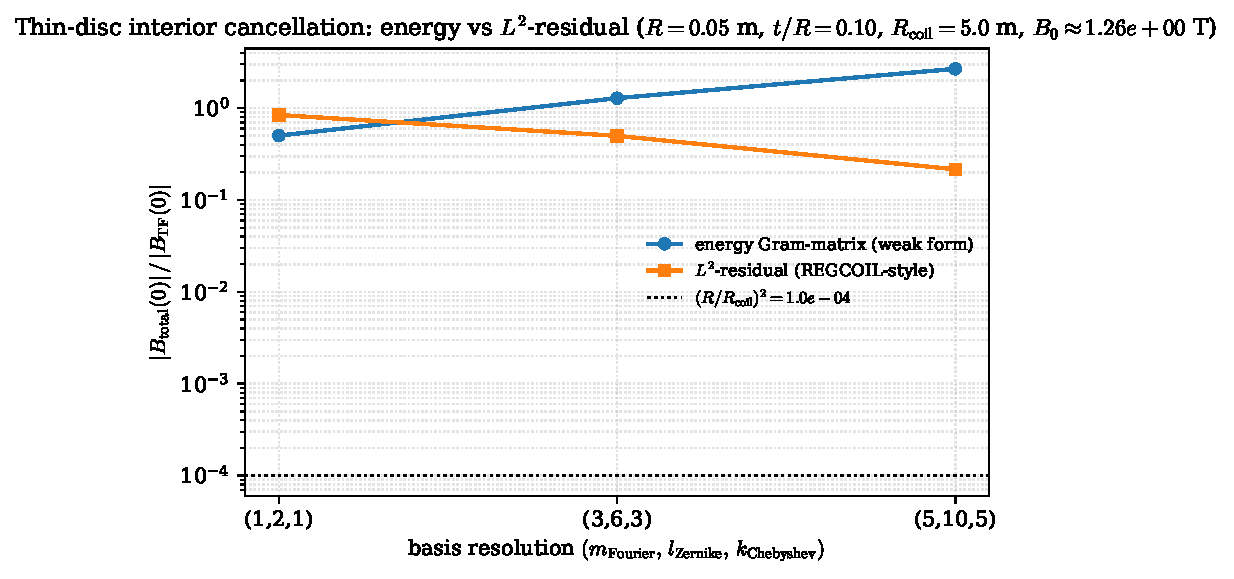
\includegraphics[width=0.75\linewidth]{figures/interior_cancellation.pdf}
  \caption{Interior field ratio
  $|\bB_{\text{tot}}(0)|/|\bB_{\text{TF}}(0)|$ vs.\ basis resolution
  for a thin puck ($R=0.05$\,m, $t/R=0.1$) in the nearly-uniform
  field of a large ring coil, comparing the energy Gram-matrix solver
  (\texttt{solver\_mode="energy"}) and the $L^2$-residual solver
  (\texttt{solver\_mode="shell\_l2"}).  The dotted line is the
  geometric ceiling $(R/R_{\rm coil})^2\approx 10^{-4}$ from TF
  non-uniformity.  The energy form does not converge in the interior
  residual (its Galerkin condition~\eqref{eq:galerkin} only constrains
  modes inside $\operatorname{span}\{\Phi_a\}$), while the $L^2$
  solver drives the ratio monotonically toward the physical floor.
  Only odd $m, k$ (with $l=2m$) are shown: for the thin-disc geometry
  the symmetric Chebyshev basis has a parity structure such that
  even-$k$ axial functions contribute negligibly to $B_n$ on the disc
  faces, and convergence is cleanest on the odd-index subsequence.}
  \label{fig:interior}
\end{figure}

\subsection{Algebraic diagnostics}
\label{sec:algebra}

\paragraph{Rim continuity residual.}
After the SVD projector $Q_c$ restricts $\mubeta$ to
$\operatorname{null}(C)$, the rim residual $\|C\mubeta\|_\infty$
should sit at round-off across resolutions.  \autoref{fig:rim} confirms
this, with the worst per-puck residual at float64 round-off
($\sim 5\times 10^{-13}$ on the finest sweep point in the figure script).

\begin{figure}[ht]
  \centering
  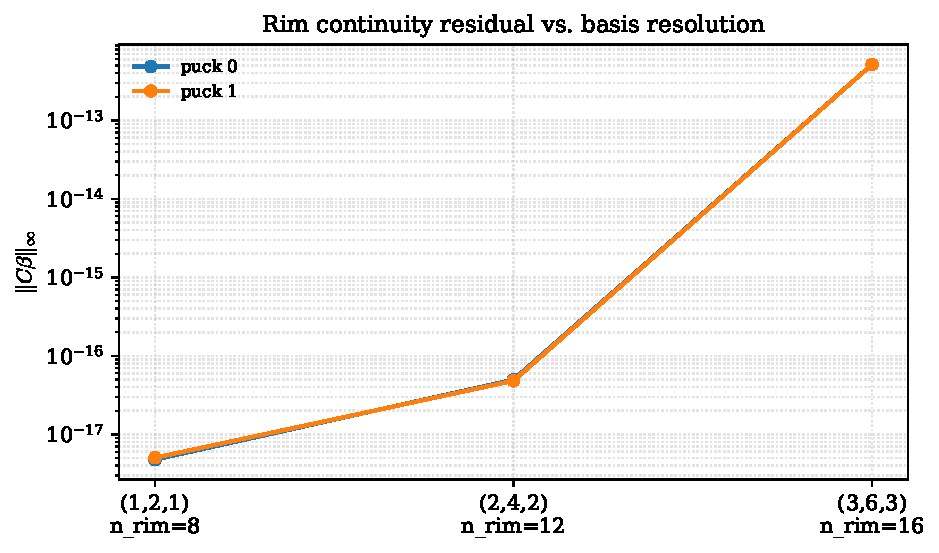
\includegraphics[width=0.65\linewidth]{figures/rim_continuity.pdf}
  \caption{$\|C\mubeta\|_\infty$ per puck vs. basis resolution: all
  values sit at float64 round-off.}
  \label{fig:rim}
\end{figure}

\paragraph{Spectrum of the reduced $L$.}
$Q_c^\top L Q_c$ is real-symmetric and positive-semidefinite
(\autoref{fig:Lspec}).  The near-null plateau at the small end of the
spectrum is the constant-$g$ gauge null space, flooded by the
eigenfloor threshold before the solve.

\begin{figure}[ht]
  \centering
  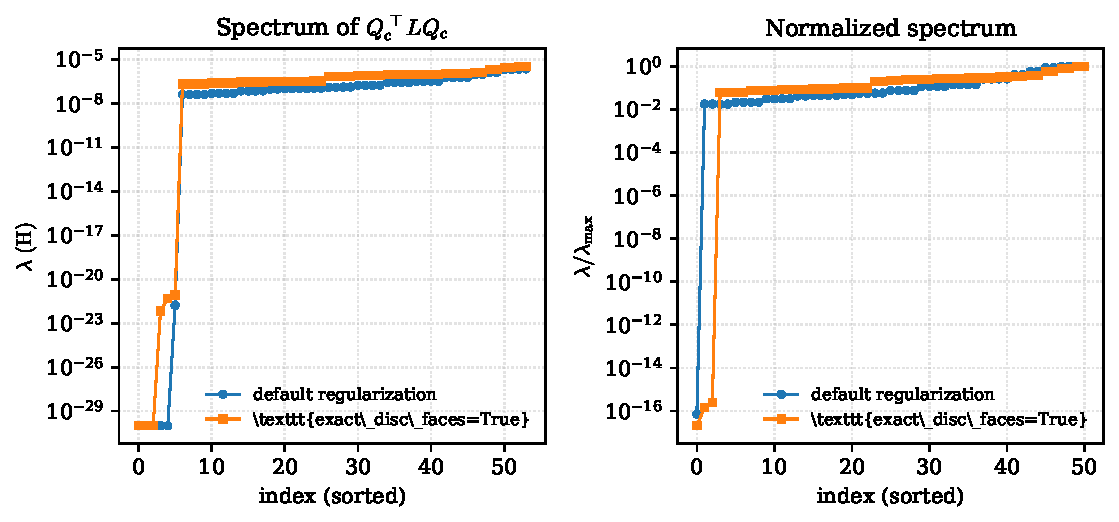
\includegraphics[width=0.95\linewidth]{figures/L_spectrum.pdf}
  \caption{Sorted eigenvalues of $Q_c^\top L Q_c$.  Left: absolute
  spectrum (H); right: normalised.  Both default regularisation and
  the \texttt{exact\_disc\_faces} path are shown.}
  \label{fig:Lspec}
\end{figure}

\subsection{Adjoint gradients (Taylor test)}
\label{sec:taylor}

For a scalar objective $J(\mathbf x)$ the central-finite-difference
directional derivative
\[
  \widetilde{\mathbf d^\top \nabla J}(\mathbf x;\epsilon)
  = \frac{J(\mathbf x + \epsilon\mathbf d) - J(\mathbf x - \epsilon\mathbf d)}{2\epsilon}
\]
must converge to $\mathbf d^\top\nabla J$ at order $\epsilon^2$.
\autoref{fig:taylor} shows this for both TF-only and TF+puck-centre
DOFs, using \fn{SquaredFlux} on a small QA surface.

\begin{figure}[ht]
  \centering
  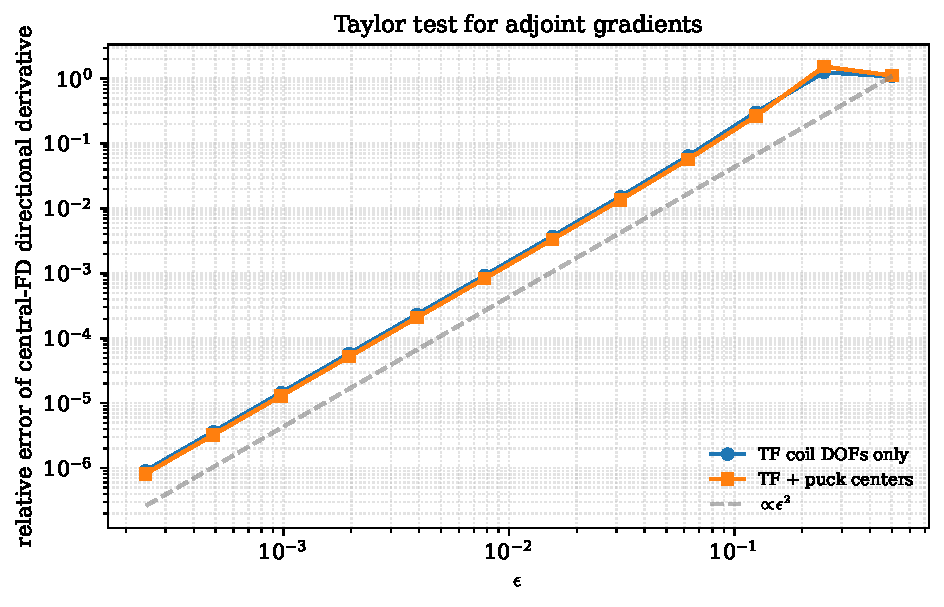
\includegraphics[width=0.70\linewidth]{figures/taylor_test.pdf}
  \caption{Taylor test: relative error of the central-FD directional
  derivative against the adjoint gradient.  The dashed line is the
  second-order reference slope.}
  \label{fig:taylor}
\end{figure}

\section{Demonstration: coupled optimisation}
\label{sec:opt}

Running L-BFGS-B on the toy setup of
\autoref{sec:taylor} (one puck, two TF coils, QA surface) with puck
geometry fixed but TF coil DOFs free reduces \texttt{SquaredFlux} by
nearly three orders of magnitude (about $740\times$) within the same
iteration budget as the figure script (\autoref{fig:opt-conv}).
Gradient flow through the implicit shell solve is correctly wired --
optimisation does not stall on a phantom gradient.

\begin{figure}[ht]
  \centering
  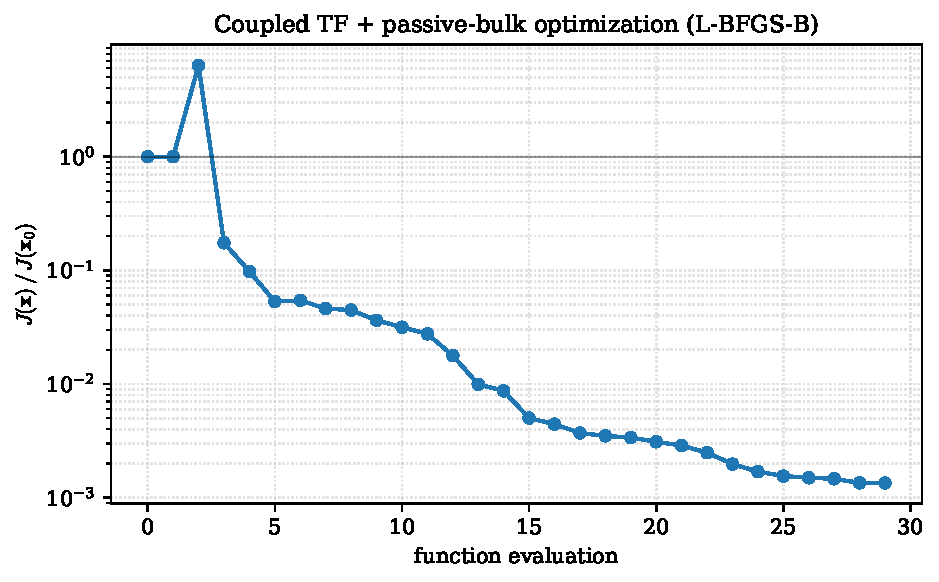
\includegraphics[width=0.70\linewidth]{figures/optimization_convergence.pdf}
  \caption{Normalised \fn{SquaredFlux} vs. function evaluation for a
  TF-coil L-BFGS-B run with the puck field coupled through the
  implicit solve.}
  \label{fig:opt-conv}
\end{figure}

\autoref{fig:pucks} shows a larger configuration (eight pucks on a
toroidal lattice around two ring coils) after the linear solve,
with the induced sheet current $|\bK|$ visualised on each puck.

\begin{figure}[ht]
  \centering
  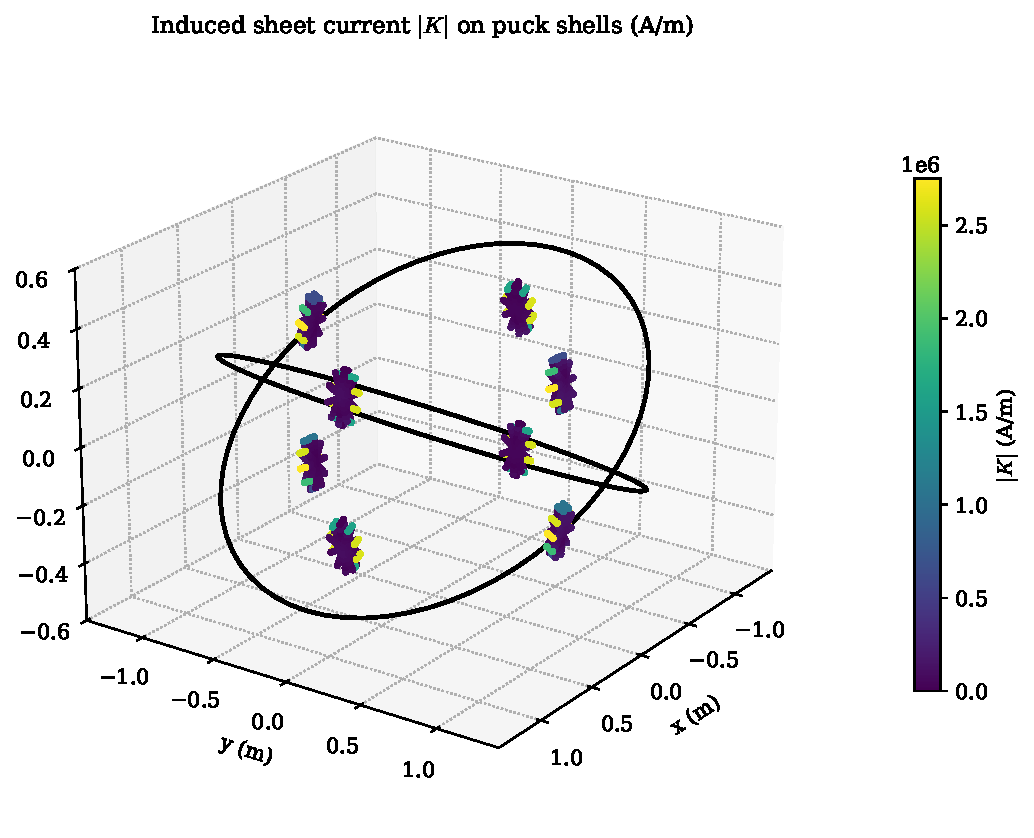
\includegraphics[width=0.80\linewidth]{figures/pucks_rendered.pdf}
  \caption{Eight passive pucks around a pair of ring TF coils; colour
  encodes $|\bK|$ (A/m) on the quadrature points of each puck (reference
  run: $\max |\bK| \approx 2.8\times 10^6$\,A/m).}
  \label{fig:pucks}
\end{figure}

For reactor-scale stellarator equilibria, the advanced examples
\file{passive\_bulks\_cylindrical\_grid\_optimization.py} and
\file{passive\_bulks\_winding\_surface\_optimization.py} (under
\file{examples/3\_Advanced/}) couple the same \texttt{SquaredFlux}
objective and TF\,+\,length penalties to optimisations where passive
bulk currents are induced at every iteration; gradients use the same
VJP path as \autoref{sec:taylor}.

\section{Known limitations}
\label{sec:limits}

\begin{itemize}
\item \fn{PassiveBulkField.\_dB\_by\_dX\_impl} raises
  \fn{NotImplementedError}; the spatial Jacobian is not yet wired.
  Any downstream consumer of $\partial \bB / \partial \mathbf x$
  (particle tracing, Boozer transforms, grad-$B$ objectives) must not
  be used with \fn{PassiveBulkField} until this is implemented.
\item VJPs with respect to per-puck $R$ and $t$ are not wired; those
  DOFs must remain fixed.  \fn{local\_unfix\_all} warns accordingly.
\item The dense $L$ matrix is $O(N_{\text{dof}}^2)$ in memory and the
  cross-block assembly is $O(N_{\text{dof}}^2\,N_{\text{quad}})$ in
  time.  This is fine for the $\sim 10$--$100$ pucks regime but not
  for grids of thousands.
\item The default \texttt{solver\_mode="energy"} formulation does not
  guarantee small pointwise interior $|\bB_{\text{tot}}|$; for
  accurate interior fields use \texttt{solver\_mode="shell\_l2"}
  (\autoref{sec:solver-modes}, \autoref{sec:interior}).  The
  \texttt{shell\_l2} path is not yet wired for free puck DOFs or the
  reduced-symmetry fast path.
\end{itemize}

\bibliographystyle{plain}
\bibliography{refs}

\end{document}
